\documentclass[12pt,a4paper]{article}
\usepackage{cmap} % Makes the PDF copiable. See http://tex.stackexchange.com/a/64198/25761
\usepackage[T1]{fontenc}
\usepackage[brazil]{babel}
\usepackage[utf8]{inputenc}
\usepackage{amsmath}
\usepackage{amsfonts}
\usepackage{amssymb}
\usepackage{amsthm}
\usepackage[usenames,svgnames,dvipsnames]{xcolor}
\usepackage{hyperref}
\usepackage{multicol}
\usepackage{graphicx}
\usepackage[margin=2cm]{geometry}

\hypersetup{
    colorlinks = true,
    allcolors = {blue}
}

% TODO: Consider using exsheets
% http://linorg.usp.br/CTAN/macros/latex/contrib/exsheets/exsheets_en.pdf
%
% http://ctan.org/tex-archive/macros/latex/contrib/exercise/
% Options: answerdelayed,lastexercise,noanswer
\usepackage[answerdelayed,lastexercise]{exercise}

\addto\captionsbrazil{%
\def\listexercisename{Lista de exerc\'icios}%
\def\ExerciseName{Exerc\'icio}%
\def\AnswerName{Solu\c{c}\~ao do exerc\'icio}%
\def\ExerciseListName{Ex.}%
\def\AnswerListName{Solu\c{c}\~ao}%
\def\ExePartName{Parte}%
\def\ArticleOf{de\ }%
}

\renewcommand{\ExerciseHeaderTitle}{(\ExerciseTitle)\ }
\renewcommand{\ExerciseListHeader}{%\ExerciseHeaderDifficulty%
\textbf{%\ExerciseListName\
\ExerciseHeaderNB.\ %
%\ --- \
\ExerciseHeaderTitle}%
%\ExerciseHeaderOrigin
\ignorespaces}
\renewcommand{\AnswerListHeader}{\textbf{\ExerciseHeaderNB.\ (\AnswerListName)\ }}

\newtheorem*{note}{Observação}
\newcommand{\fixme}{{\color{red}(...)}}
\newcommand*\diff{\mathop{}\!\mathrm{d}}
\newcommand*\sen{\operatorname{sen}}
\newcommand*\tg{\operatorname{tg}}
\newcommand*\cotg{\operatorname{cotg}}
\newcommand*\cosec{\operatorname{cossec}}
\newcommand*\cotgh{\operatorname{cotgh}}
\newcommand*\arcsen{\operatorname{arcsen}}
\newcommand*\arctg{\operatorname{arctg}}
\newcommand*\abs[1]{\left|#1\right|}
\newcommand*\R{\mathbb{R}}
\newcommand*\op[1]{\overset{#1}{\rightarrow}}

\renewcommand{\theenumi}{\alph{enumi}}
\renewcommand\labelenumi{(\theenumi) }

\newcommand*\tipo{Prova I}
\newcommand*\turma{CIV241-02U}
\newcommand*\disciplina{CDI2002}
\newcommand*\eu{Helder G. G. de Lima}
\newcommand*\data{12/09/2024}

\author{\eu}
\title{\tipo - \disciplina}
\date{\data}

\begin{document}
\thispagestyle{empty}
\newgeometry{margin=2cm,bottom=0.5cm}
\begin{center}

\includegraphics[width=9.0cm]{marca} \\
\textbf{\tipo\ (\disciplina / \turma)} \\
Prof. \eu\footnote{
Este é um material de acesso livre distribuído sob os termos da licença \href{https://creativecommons.org/licenses/by-sa/4.0/deed.pt_BR}{Creative Commons BY-SA 4.0}}
\end{center}

\noindent Nome do(a) aluno(a): \underline{\hspace{9,7cm}} Data: \underline{\data}

\begin{center}\fbox{
\begin{minipage}{14cm}

{\footnotesize
\begin{itemize}
\renewcommand{\theenumi}{\Roman{enumi}}
\item Identifique-se em todas as folhas.
\item Mantenha o celular e os demais equipamentos eletrônicos desligados durante a prova.
\item Justifique cada resposta com cálculos ou argumentos baseados na teoria estudada.
\item Resolva $4$ das $5$ questões (deixe claro que questão não deverá ser corrigida).
\end{itemize}
}

\end{minipage}
}
\end{center}

\begin{ExerciseList}
\Exercise[title={2,5}] Calcule a integral definida $\displaystyle\int_{-\sqrt{2}/2}^{\sqrt{2}/2} \frac{2x^2-1}{\sqrt{1-x^2}} \diff{x}$.
\Answer \textbf{Solução 1}: Fazendo a substituição trigonométrica $x = \sen(\theta)$, tem-se $\diff{x} = \cos(\theta) \diff{\theta}$ e para $x=\pm \sqrt{2}/2$ tem-se $\theta=\pm \pi/4$. Então
\begin{align*}
  \int_{-\sqrt{2}/2}^{\sqrt{2}/2} \frac{2x^2-1}{\sqrt{1-x^2}} \diff{x}
  & = \int_{-\pi/4}^{\pi/4} \frac{2\sen^2(\theta)-1}{\sqrt{1-\sen^2(\theta)}} \cos(\theta) \diff{\theta}
  = \int_{-\pi/4}^{\pi/4} \frac{2\sen^2(\theta)-1}{\sqrt{\cos^2(\theta)}} \cos(\theta) \diff{\theta}\\
  & = \int_{-\pi/4}^{\pi/4} \frac{2\sen^2(\theta)-1}{|\cos(\theta)|} \cos(\theta) \diff{\theta}
  = \int_{-\pi/4}^{\pi/4} \frac{2\sen^2(\theta)-1}{\cos(\theta)} \cos(\theta) \diff{\theta}\\
  & = \int_{-\pi/4}^{\pi/4} 2\sen^2(\theta)-1 \diff{\theta}
    = \int_{-\pi/4}^{\pi/4} 2\left[\frac{1}{2}\left(1-\cos(2\theta)\right)\right]-1 \diff{\theta}\\
  & = \int_{-\pi/4}^{\pi/4} -\cos(2\theta) \diff{\theta}
    = -\frac{\sen(2\theta)}{2}\bigg|_{-\pi/4}^{\pi/4}
    = -\frac{\sen(\pi/2)}{2} + \frac{\sen(-\pi/2)}{2}
    = -1.
\end{align*}

\textbf{Solução 2}: Considerando que a função é par, é possível obter a mesma resposta duplicando o valor da integral
$\displaystyle\int_{0}^{\sqrt{2}/2} \frac{2x^2-1}{\sqrt{1-x^2}} \diff{x}$.

\textbf{Solução 3}: Também é possível calcular a integral utilizando a substituição trigonométrica $x = \cos(\theta)$, que resulta em $\diff{x} = -\sen(\theta)\diff{\theta}$, com $\theta \in [\frac{\pi}{4}, \frac{3\pi}{4}]$.

\Exercise[title={2,5}] Calcule, caso seja convergente, a integral imprópria $\displaystyle\int_2^5 \frac{2}{\sqrt{3x-6}} \diff{x}$.
\Answer Observe que a função $f(x) = \frac{2}{\sqrt{3x-6}}$ não está definida em $x=2$:
\begin{center}
\includegraphics[width=6.5cm]{img/2-integral-imprópria.pdf}
\end{center}

Tem-se:
\[
  \int_2^5 \frac{2}{\sqrt{3x-6}} \diff{x}
  = \lim_{t\to 2^+} \int_t^5 \frac{2}{\sqrt{3x-6}} \diff{x}.
\]

\textbf{Solução 1}: Fazendo a mudança de variável $u = 3x - 6$, tem-se $x = \frac{u+6}{3}$ e $\diff{x} = \frac{1}{3} \diff{u}$. Além disso, para $x=t$, tem-se $u = 3t-6$ e para $x=5$ tem-se $u=9$, então:
\begin{align*}
  \int_2^5 \frac{2}{\sqrt{3x - 6}} \diff{x}
  & = \lim_{t\to 2^+} \int_{3t - 6}^9 \frac{2}{\sqrt{u}} \frac{1}{3}\diff{u}
  = \lim_{t\to 2^+} \frac{2}{3} \int_{3t - 6}^9 u^{-\frac{1}{2}} \diff{u}
  = \lim_{t\to 2^+} \frac{2}{3} (2u^{\frac{1}{2}})\bigg|_{3t - 6}^9\\
  & = \lim_{t\to 2^+} \frac{2}{3} (2\cdot \sqrt{9} - 2\cdot \sqrt{3t - 6})
  = \frac{2}{3} (6 - 0)
  = 4.
\end{align*}

\textbf{Solução 2}: Outra opção é utilizar a mudança de variável $v = \sqrt{3x-6}$, obtendo $\diff{v} = \frac{3}{2\sqrt{3x-6}}\diff{x}$, $v=3$ para $x=5$ e $v=\sqrt{3t-6}$ para $x=t$, de modo que
\begin{align*}
  \int_2^5 \frac{2}{\sqrt{3x - 6}} \diff{x}
  &
  = \lim_{t\to 2^+} \int_t^5 \frac{4}{3} \cdot \frac{3}{2\sqrt{3x-6}} \diff{x}
  = \lim_{t\to 2^+} \int_{\sqrt{3t-6}}^3 \frac{4}{3} \diff{v}
  = \lim_{t\to 2^+} \frac{4}{3}v\bigg|_{\sqrt{3t-6}}^3\\
  & = \lim_{t\to 2^+} \frac{4}{3} (3 - \sqrt{3t-6})
  = \frac{4}{3} (3 - 0)
  = 4.
\end{align*}

\Exercise[title={2,5}] Calcule a área da região simultaneamente interior às circunferências cujas equações em coordenadas polares são \(r = 4\cos(\theta)\) e \(r = 4\sen(\theta)\):

\includegraphics[width=7.0cm]{img/circunferências.pdf}

\Answer \textbf{Solução 1}: Cada um dos pontos \((r, \theta)\) da região hachurada têm ângulo
$\theta \in [0, \pi/2]$. No entanto, como a região é simétrica em relação à reta $\theta = \pi/4$, pode-se considerar os pontos com $\theta \in [0, \pi/4]$ e raio $r \in [0, 4\sen(\theta)]$. Logo, a área $A$ da região é dada por
\begin{align*}
  A
  & = 2 \cdot \left( \frac{1}{2}\int_0^{\pi/4} \left(4 \sen(\theta)\right)^2 \diff\theta\right)
    = \int_0^{\pi/4} 16 \sen^2(\theta) \diff\theta
    = \int_0^{\pi/4} 16 \cdot \left(\frac{1}{2}\left(1-\cos(2\theta)\right)\right) \diff\theta \\
  & = \int_0^{\pi/4} 8 + 8\cos(2\theta) \diff\theta
    = \left(8\theta - 4\sen(2\theta) \right)\big\rvert_0^{\pi/4} \\
  & = \left(8\cdot\frac{\pi}{4} - 4\sen\left(2\cdot\frac{\pi}{4}\right)\right)
    - \left(8\cdot0 - 4\sen\left(2\cdot0\right)\right)
    = 2\pi - 4 \text{ u.a.}.
\end{align*}

\textbf{Solução 2}: Outra alternativa é considerar separadamente $\theta \in [0, \frac{\pi}{4}]$ e $\theta \in [\frac{\pi}{4}, \frac{\pi}{2}]$ e calcular:
\[
A
= \frac{1}{2}\int_0^{\pi/4} \left(4 \sen(\theta)\right)^2 \diff\theta
+ \frac{1}{2}\int_{\pi/4}^{\pi/2} \left(4 \cos(\theta)\right)^2 \diff\theta.
\]


\Exercise[title={2,5}] Calcule o comprimento de arco da função $f(x) = \ln(\cos(x))$ no intervalo $\left[0,\frac{\pi}{3}\right]$.
\Answer Como $f^\prime(x) = \frac{1}{\cos(x)}\cdot (-\sen(x)) = -\tan(x)$, tem-se:
\[
\sqrt{1+[f^\prime(x)]^2}
= \sqrt{1+\tan^2(x)}
= \sqrt{\sec^2(x)}
= |\sec(x)|
= \sec(x), \text{ se } x \in \left[0,\frac{\pi}{3}\right].
\]
Logo, o comprimento de arco é
\begin{align*}
  L
  & = \int_0^{\pi/3} \sec(x) \diff{x}
  = \ln|\sec(x)+\tan(x)|\bigg|_0^{\pi/3}
  = \ln|\sec(\pi/3)+\tan(\pi/3)| - \ln|\sec(0)+\tan(0)| \\
  & = \ln|2 + \sqrt{3}| - \ln|1 + 0|
  = \ln(2 + \sqrt{3}).
\end{align*}


\Exercise[title={2,5}] Considere a função integrável $f:[-3, 0] \to [0, 10]$ dada por $f(x) = 10 - x^2$. Utilize um limite de somas inferiores para calcular a integral definida $\int_{-3}^0 f(x) \diff{x}$.

\begin{center}
Lembrete:
\(
  1 + 2 + \cdots + n = \dfrac{n(n+1)}{2}
\)
e
\(
  1^2 + 2^2 + \cdots + n^2 = \dfrac{n(n+1)(2n+1)}{6}
\)
.
\end{center}
\Answer A resolução consistirá das seguintes etapas:
\begin{itemize}
  \item Obter uma partição do intervalo $[-3, 0]$ com $n$ subintervalos de mesmo comprimento
  \item Identificar em que extremidade de cada intervalo a função assume seu valor mínimo (pois devem ser usadas somas inferiores)
  \item Expressar a soma inferior correspondente à partição obtida em termos de $n$
  \item Obter a integral como um limite da soma inferior quando $n$ tende a infinito
\end{itemize}

Seja $P = \{ x_0, \ldots, x_n \}$ a partição do intervalo $[-3, 0]$ em $n$ subintervalos de mesmo comprimento $\Delta x = \frac{3}{n}$, isto é,
\[
  x_0 = -3,\quad
  x_1 = -3 + \Delta x,\quad
  x_2 = -3 + 2\Delta x,\quad
  \quad\ldots,\quad
  x_n = -3 + n\Delta x = 0.
\]

Como $f$ é uma função crescente (pois sua derivada $f^\prime(x) = -2x > 0$ para $x \in [-3, 0]$), o valor mínimo de $f$ em cada subintervalo $[x_{i-1}, x_i]$ é alcançado na extremidade esquerda, $x_{i-1}$. A figura a seguir mostra o caso em que $n = 3$:
\begin{center}
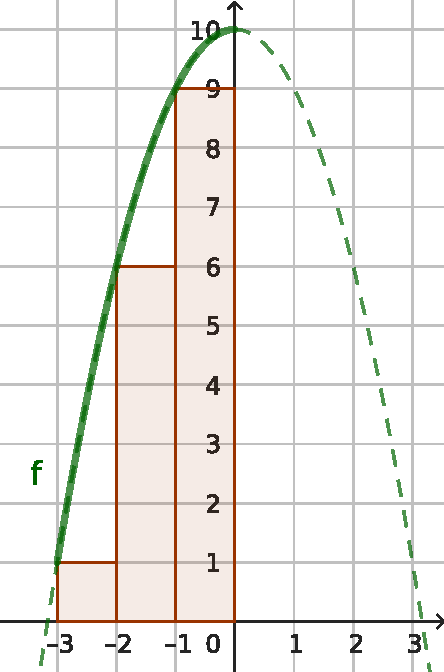
\includegraphics[width=5.0cm]{img/soma-inferior.pdf}
\end{center}
Deste modo, a soma inferior correspondente à partição $P$ é:
\begin{align*}
  \underline{S}(f, P)
  & = \sum_{i=0}^{n-1} f(x_i) \Delta x
    = \sum_{i=0}^{n-1} \left(10-x_i^2\right) \Delta x
    = \sum_{i=0}^{n-1} \left(10-(-3 + i\Delta x)^2\right) \Delta x \\
  & = \sum_{i=0}^{n-1} \left(10-(9 - 6i\Delta x + i^2(\Delta x) ^2)\right) \Delta x
    = \sum_{i=0}^{n-1} \left(1 + 6i\Delta x - i^2(\Delta x) ^2)\right) \Delta x \\
  & = \sum_{i=0}^{n-1} \Delta x + 6i(\Delta x)^2 - i^2(\Delta x) ^3
    = \sum_{i=0}^{n-1} \frac{3}{n}\
    + 6i\left(\frac{3}{n}\right)^2
    - i^2\left(\frac{3}{n}\right)^3 \\
  & = n\cdot \left(\frac{3}{n}\right)
    + 6 \left(\frac{3}{n}\right)^2 \cdot \sum_{i=0}^{n-1} i
    - \left(\frac{3}{n}\right)^3 \cdot \sum_{i=0}^{n-1} i^2 \\
  & = 3
    + \frac{54}{n^2} \left(\frac{(1+(n-1))(n-1)}{2}\right)
    - \frac{27}{n^3}\left(\frac{(n-1)((n-1)+1)(2(n-1)+1)}{6}\right) \\
  & = 3
    + \frac{54}{n^2} \left(\frac{n^2 - n}{2}\right)
    - \frac{27}{n^3}\left(\frac{2 n^3 - 3 n^2 + n}{6}\right)
    = 3 + (27 - 27n)
    - \left(\frac{9}{2 n^2} - \frac{27}{2 n} + 9\right) \\
  & = 21 - \frac{27}{2 n} -\frac{9}{2 n^2}.
\end{align*}

Logo, $\int_{-3}^0 10-x^2\diff{x} = \lim_{n \to \infty} 21 - \frac{27}{2 n} -\frac{9}{2 n^2} = 21$.

\begin{note}
  Pode-se validar a resposta obtida calculando a mesma integral por meio do teorema fundamental do cálculo:
  \[
    \int_{-3}^0 10-x^2\diff{x}
    = \left(10x-\frac{x^3}{3}\right)\bigg\rvert_{-3}^0
    = \left(10 \cdot 0-\frac{0}{3}\right) - \left(-30 - \frac{-27}{3}\right)
    = 21.
  \]
\end{note}
\end{ExerciseList}

\vfill
\begin{center}
BOA PROVA!
\end{center}

\newpage
\restoregeometry
\section*{Respostas}
\shipoutAnswer
\end{document}
